\section{MTT Simulation Studies}
For future physics studies with MTT this system has to be implemented in the standard CMS geometry description within CMSSW, the software framework of CMS.
In this section the implementation of MTT in CMS is described.
\subsection{MTT Geometry in CMSSW}
	\subsubsection{The geometry model of CMS}
	The geometry model of CMS is based on Geant4 (REF).
	It is constructed hierarchically and realized by the XML based detector description language (REF).
	To make the geometry available on runtime the ESProducer \textbf{XMLIdealGeometryESSource} is used converting the XML description of the geommetry in a C++ model.
	The tree structure of the geometry is then available as an instance of the \textbf{DDCompactView}.
	In general there are two main classes of geometries existent in CMS.
	For the tracking systems like the muon subdetectors and tracker etc. tracking geometries are available.
	For the calorimeter systems one can use the caloriemeter geometry classes.
	Details on this procedure can be found in (REF).
	For alternative geometry models like the extended CMS geometry containing the MTT system it is nessessary to modify the ESProducer to load corresponding XML files.
	In the next section the XML file of the MTT system is explained.
	\subsubsection{Description of the MTT geometry for different scenarios}
		\subsubsection*{General:}
		All parts of the MTT geometry are arranged in a hierarchy which is very similar to the geometry hierarchy of the muon system, especially the DT system.
		This means that the MTT geometry is to be assigned to the class of tracking geometries.
		Furthermore the local coordinate system of the MTT is chosen in a way, that the z axis concurs with the global z axis of the CMS.
		The local y axis therefore is pointing outwards radially.
		\subsubsection*{Inner Hierarchy:}
		The basic unit of the MTT geometry is the \textbf{MTTTile}.
		This unit is consisting of a scintillator of 10\,mm thickness wrapped by a polyethylene layer of 1\,mm thickness.
		In figure \ref{fig:tile_wowrapping}
		The sensitive material of the scintillator is a generic hydrogencarbon compound with the mass composition of $m_H:m_C \approx 91,5\%:8,5\%$.
		\begin{figure}[htbp]
			\centering
			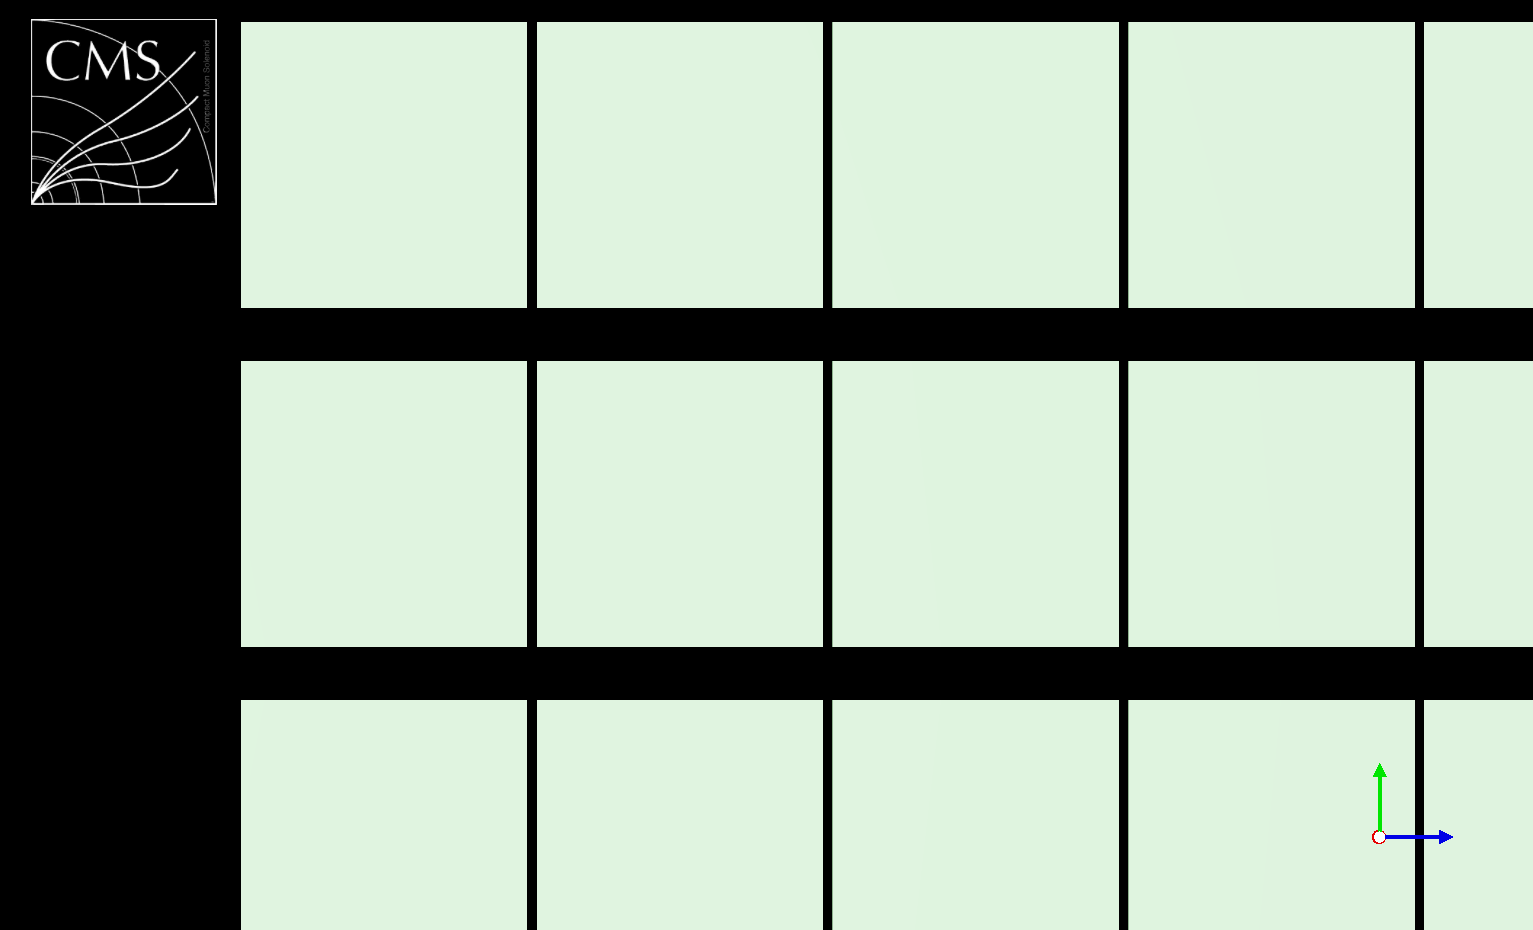
\includegraphics[width=0.6\textwidth]{Figures/erdogan/tile_wowrapping.png}
			\caption{MTT geometry: tiles without their wrappings.}
			\label{fig:tile_wowrapping}
		\end{figure}
		Several MTTTiles can be arranged along the z axis in a \textbf{MTTStrip} (figure \ref{fig:strip}).
		\begin{figure}[htbp]
			\centering
			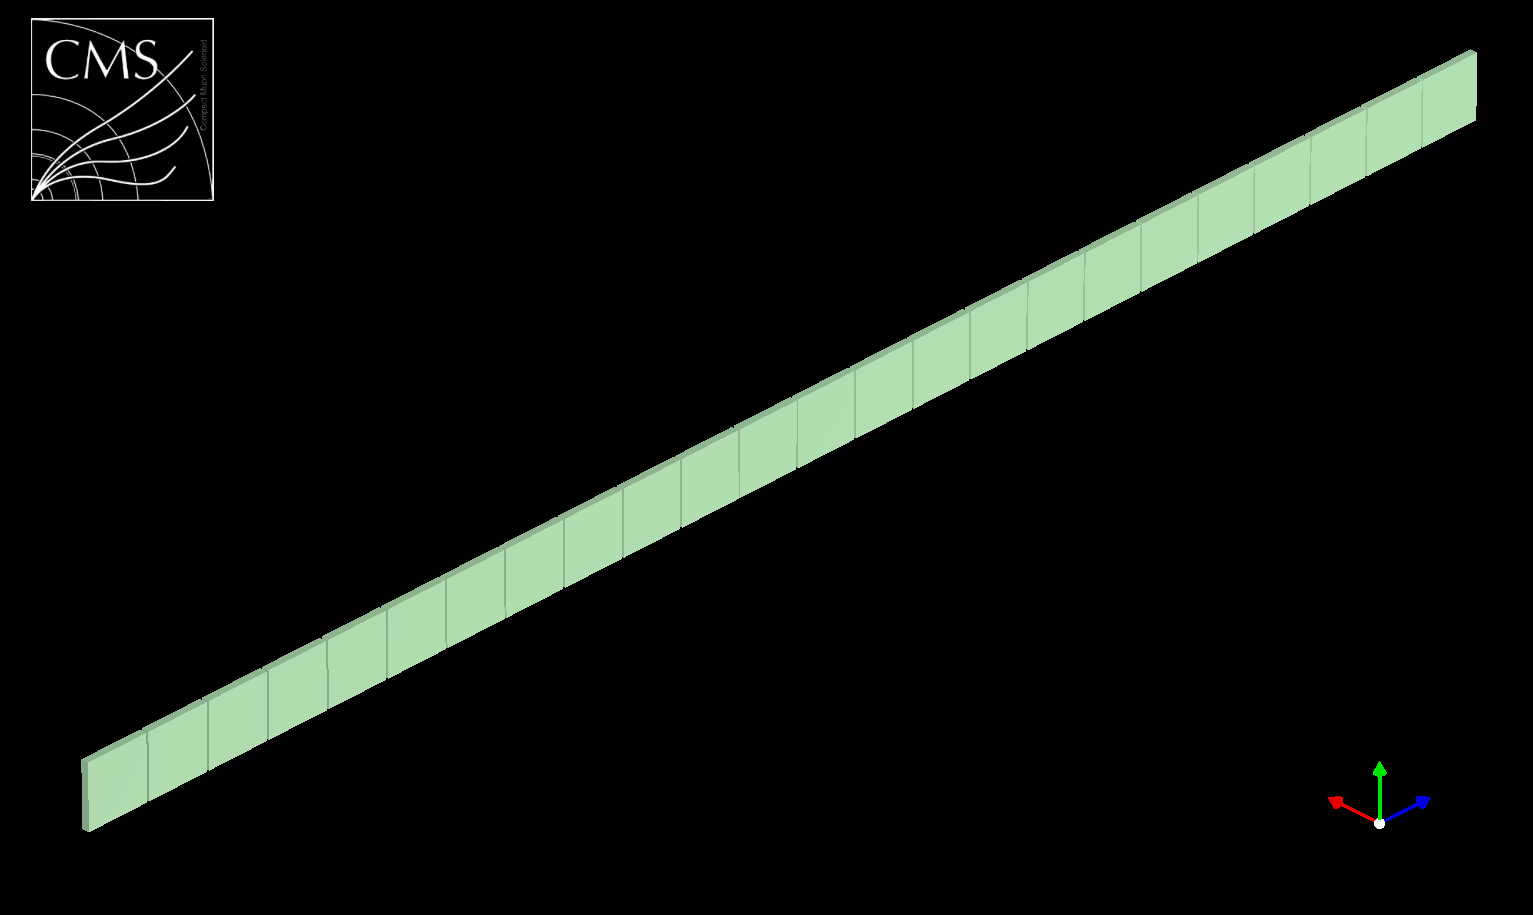
\includegraphics[width=0.6\textwidth]{Figures/erdogan/strip.png}
			\caption{MTT geometry: array of several tiles = strip.}
			\label{fig:strip}
		\end{figure}
		The dimensions of the tiles are dynamic and determined automatically to be fit in a MTTStrip in a way that a strip contains the number of tiles given by the user having the insensitive areas
		between the tiles to be minimal.
		However the dimension of a strip is in z direction fixed at 2536\,mm since this is the width of the wheels. 
		The strip itself is made of polystrene.
		An array of strips in local x direction is called a layer (figure \ref{fig:layer}).
		\begin{figure}[htbp]
			\centering
			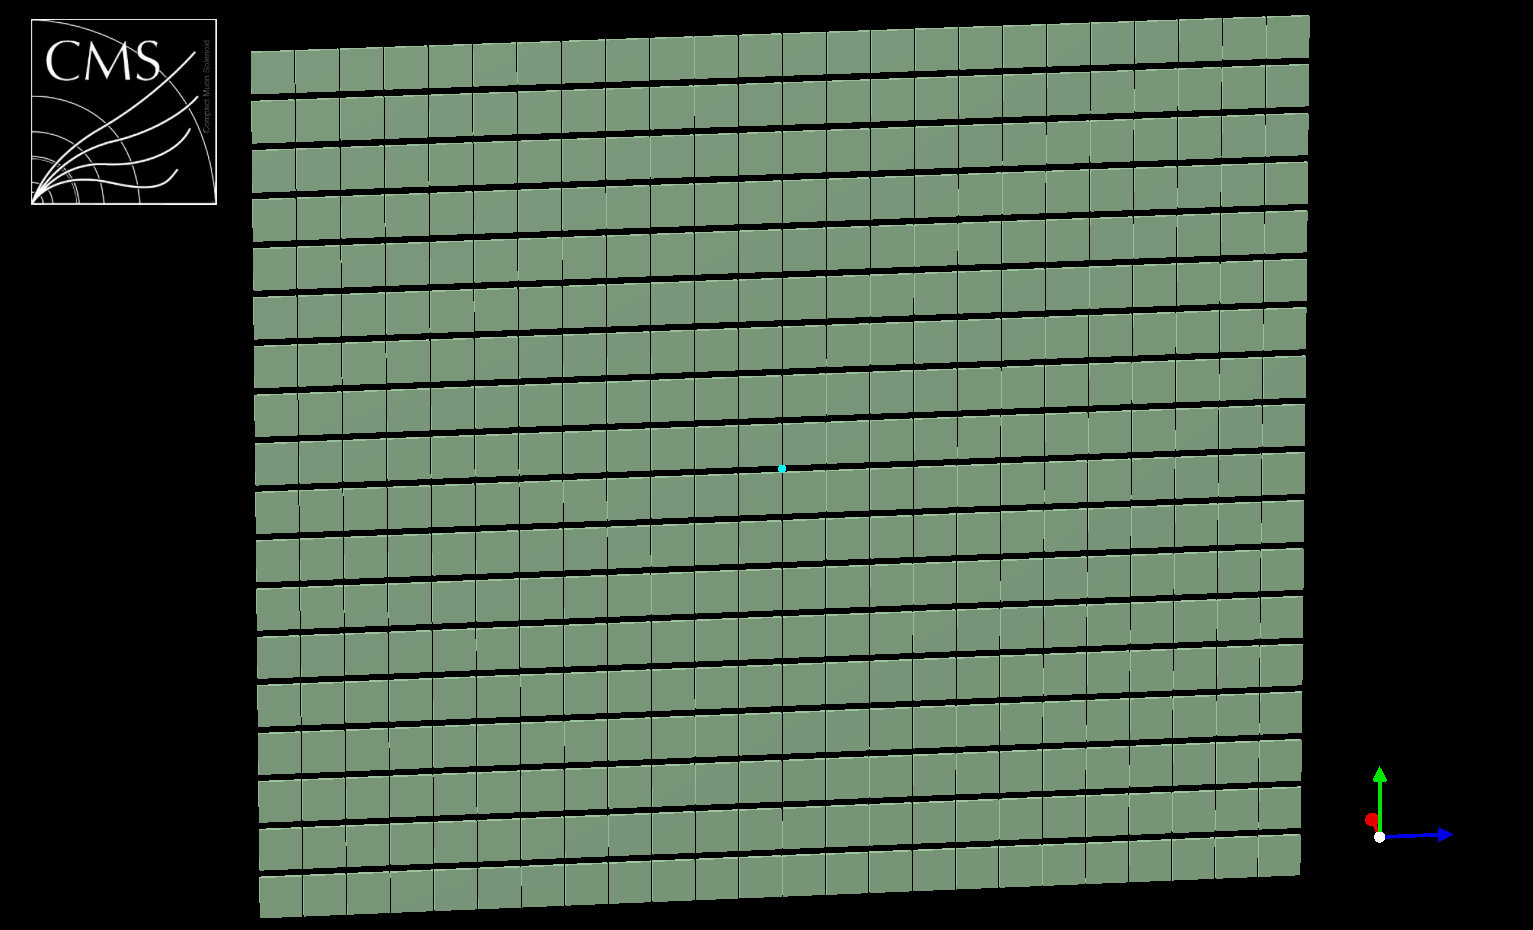
\includegraphics[width=0.6\textwidth]{Figures/erdogan/layer.png}
			\caption{MTT geometry: array of several strips = layer.}
			\label{fig:layer}
		\end{figure}
		Several layers in y direction than can be arranged in a panel which is the top unit in the hierarchy.
		There are already several scenarios written for MTT geometry having one layer in a panel or more layers (figure \ref{fig:panel}).
		\begin{figure}[htbp]
			\centering
			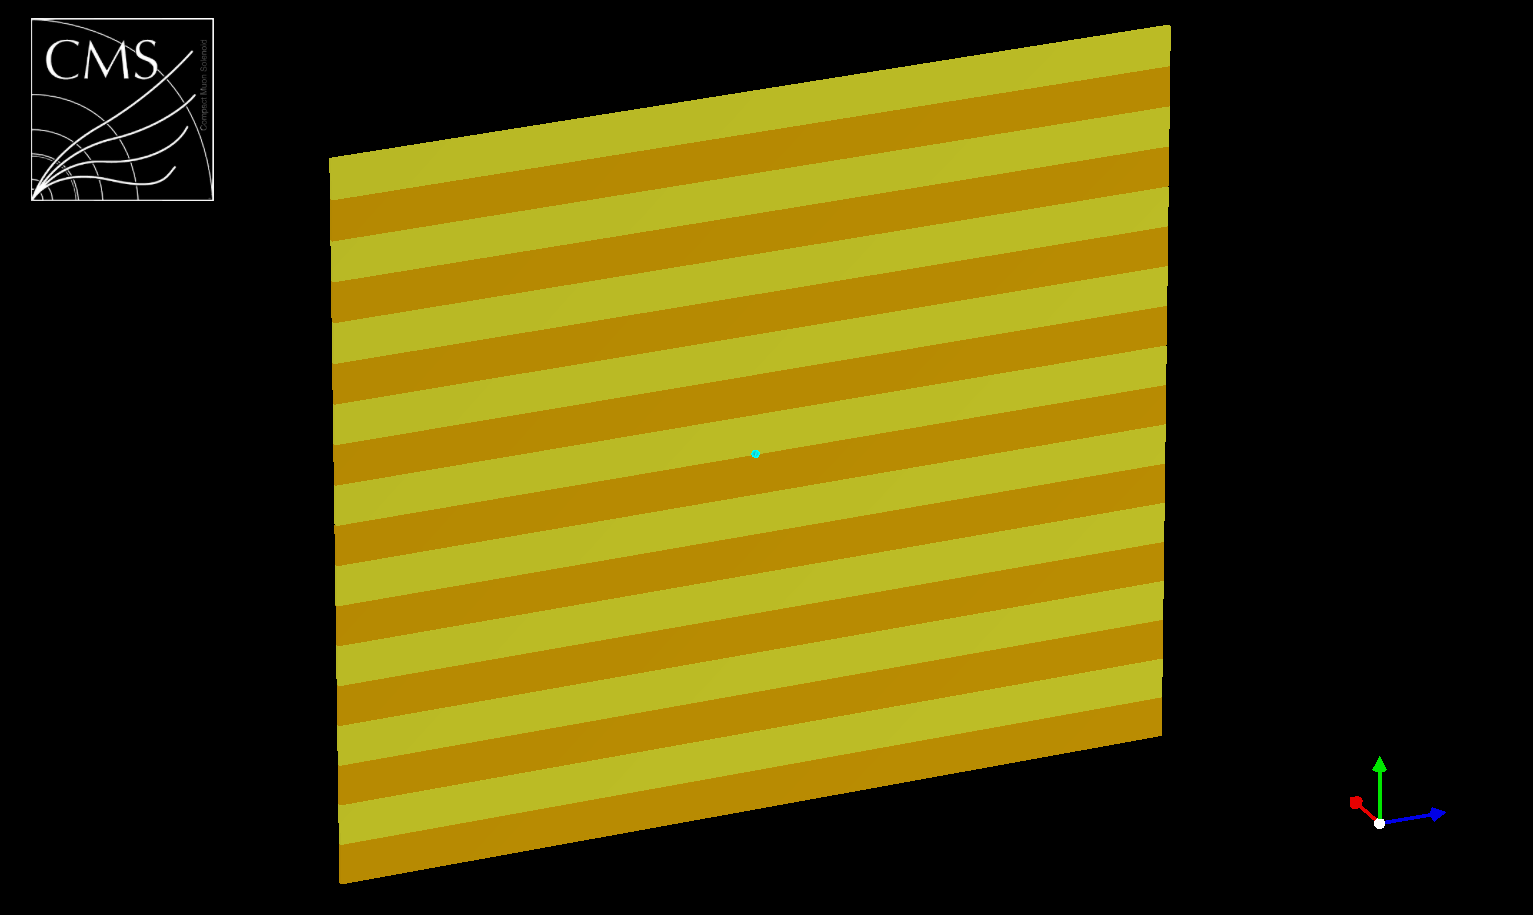
\includegraphics[width=0.45\textwidth]{Figures/erdogan/panel1.png}
			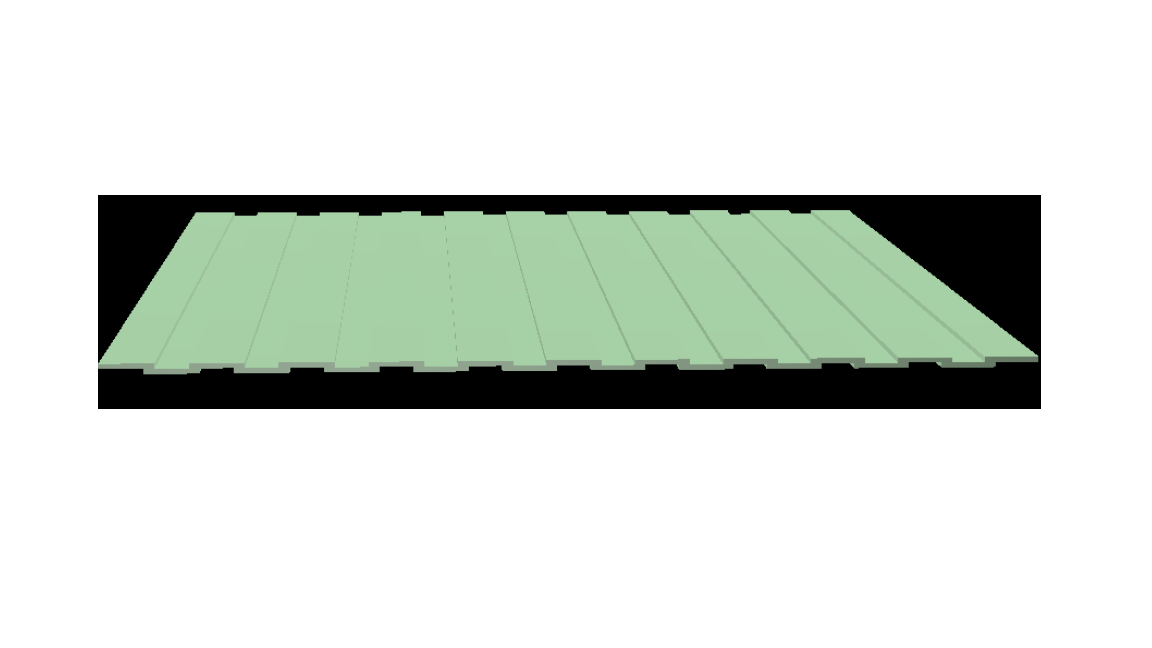
\includegraphics[width=0.45\textwidth]{Figures/erdogan/panel2.png}
			\caption{left one MTT panel with one layer, right a possible scenario for one panel with two layers}
			\label{fig:panel}
		\end{figure}
		\subsubsection*{Numbering:}
		In CMS detector description each detector unit is unique by a 32 bit integer named the DetId.
		The composition of this integer is depicted in figure \ref{fig:numbering}.
		\begin{figure}[htbp]
			\centering
			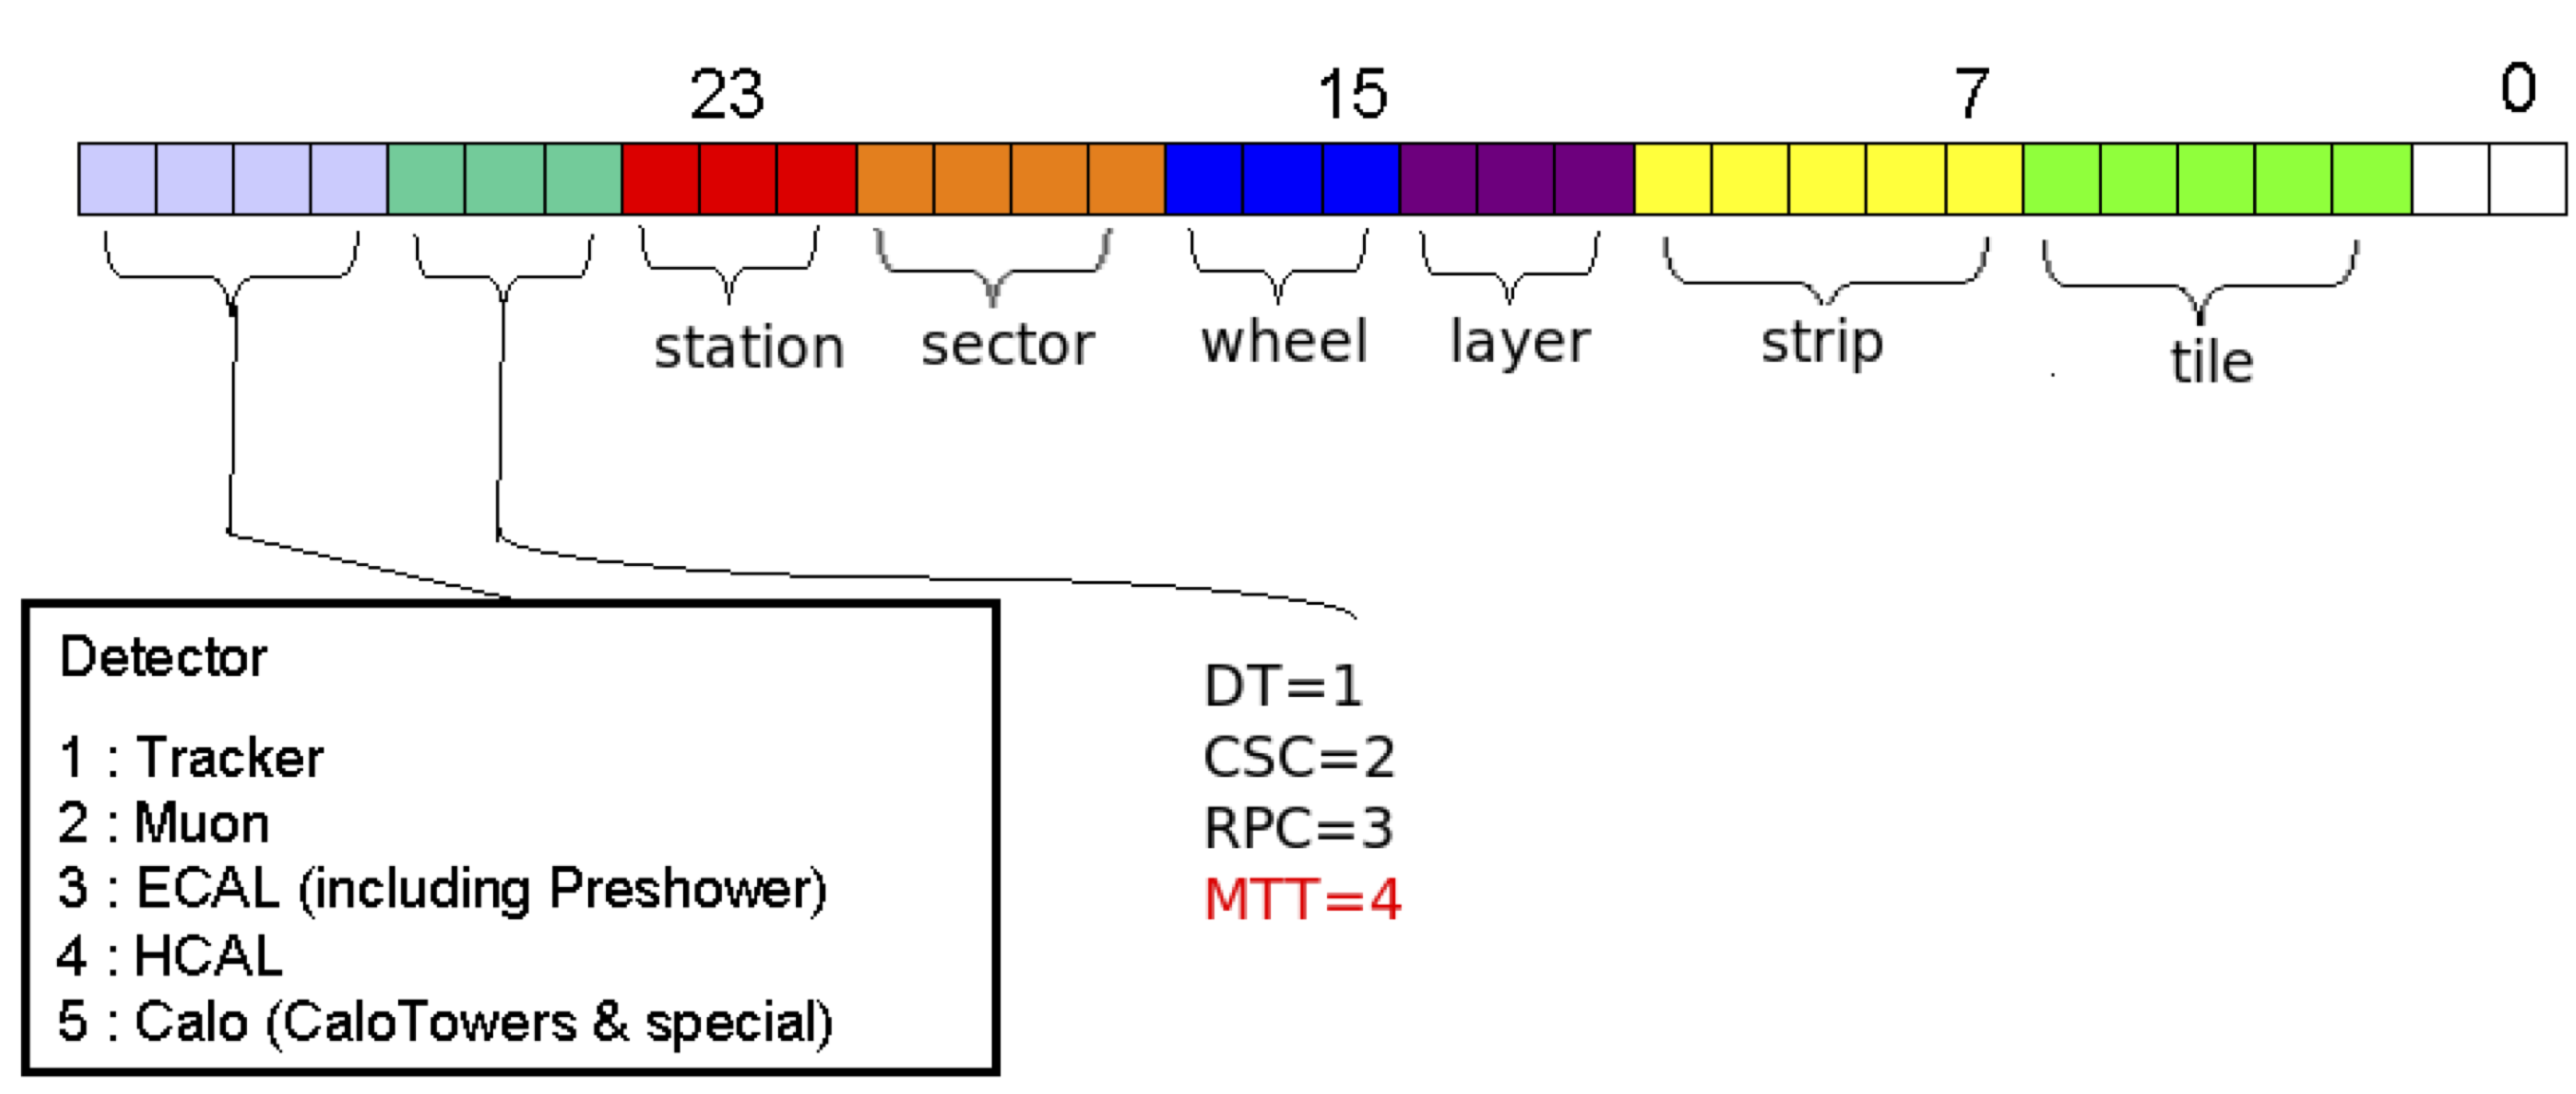
\includegraphics[width=0.6\textwidth]{Figures/erdogan/numbering.png}
			\caption{numbering scheme of MTT detectors.}
			\label{fig:numbering}
		\end{figure}
		The first 4 bits are reserved for the subdetector to which the considered detector unit belongs to.
		Following 3 bits are marking the subsystem within the subdetector, like DT,CSC,RPC or in our case MTT within the muon system.
		The remaining bits are to desribe the location of the detector unit in a certain wheel, station etc.
		For MTT we used the 3 bits after the bits for the subsystem, for the station, 4 bits for the sector, 3 bits for the wheel, 3 bits for the layer, 5 bits for the strip and 5 bits for the tile.
		With this a MTT system consisting of 7 layers each with 31 strips per $\phi$-sector can be numbered consecutively in a unique way.
		This would allow tiles with only a few $cm^2$ surface area and since the planned MTT tiles are around $10x10\,cm^2$ this numbering is more than sufficient.
	\subsubsection{Setup for the SimHit generation}
		After having the geometry of MTT within the CMSSW the next step is to create tools to simulate hits when particles go through a MTT tile.
		This task is handled by the MTTSensitiveDetector tool which is based on the Geant4 counterpart SensitiveDetector.
		It collects information like energy loss or time of flight from the Geant4 step where a particle track goes through the sensitive detector.
		Having this tool the general hit producer within CMSSW named OscarProducer which is responsible for producing hits 
		the producer for simulated hits has to be trained to consider also hits from the MTT system.
		This producer is called the OscarProducer  
	\subsubsection{DIGI generation}
	\subsubsection{to do}
\subsection{First SimHit studies and their results}
	All in this section shown first results are described in detail in (PAULREF).
